\subsubsection{Q10.20 data 09202021 10082021 10312021 11092021 grouped by scenario \& Sex}

\begin{comment}
                            EFPR        EO      EFNR     n    pvalue
(frauth, DATA EXPIRED)  0.000000  1.000000  0.000000   1.0  1.000000
(frauth, Female)        0.527273  0.472727  0.509091  55.0  0.644689
(frauth, Male)          0.428571  0.571429  0.404762  21.0  0.592980
(icu, Female)           0.566038  0.433962  0.613208  53.0  0.178289
(icu, Male)             0.545455  0.454545  0.636364  11.0  0.525394
(rent, Female)          0.479167  0.520833  0.468750  48.0  0.862032
(rent, Male)            0.375000  0.625000  0.375000  24.0  0.232165
\end{comment}

\begin{table}[h]
    \centering
    \begin{tabular}{|c|c|c|c|c|c|c|}
        \hline
        scenario & Sex & EFPR & EO & EFNR & n & p-value\\
        \hline
        frauth & DATA EXPIRED & 0.000 & \textbf{1.000} & 0.000 & 1.0 & 1.000\\
		frauth & Female & \textbf{0.527} & 0.473 & \textbf{0.509} & 55.0 & 0.645\\
		frauth & Male & 0.429 & \textbf{0.571} & 0.405 & 21.0 & 0.593\\
		icu & Female & \textbf{0.566} & 0.434 & \textbf{0.613} & 53.0 & 0.178\\
		icu & Male & \textbf{0.545} & 0.455 & \textbf{0.636} & 11.0 & 0.525\\
		rent & Female & 0.479 & \textbf{0.521} & 0.469 & 48.0 & 0.862\\
		rent & Male & 0.375 & \textbf{0.625} & 0.375 & 24.0 & 0.232\\
		
        \hline
    \end{tabular}
    \caption{Grouped by scenario Sex}
    \label{tab:my_label}
\end{table}
\begin{figure}[h]
    \centering
    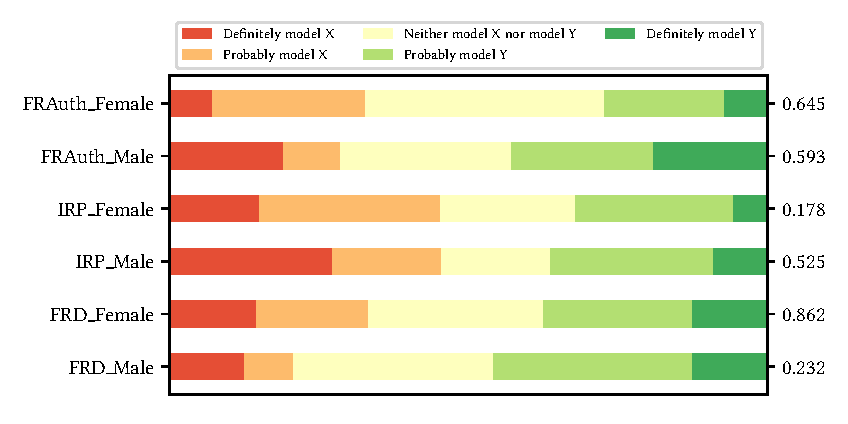
\includegraphics[width=0.8\textwidth]{figures/Q10.20/09202021_10082021_10312021_11092021/Q10.20_scenario_Sex.pdf}
    \caption{Grouped by scenario \& Sex}
    \label{fig:my_label}
\end{figure}
